\documentclass[aspectratio=169, table]{beamer}

\graphicspath{{../../images/}}

%\usepackage[beamertheme=./praditatheme]{Pradita}

\usetheme{Pradita}

\title{\huge Chapter-14:\\DevOps}
\subtitle{IF231303-Software Architecture}
\author{Hendra Lijaya, Oktavianus Hendry Wijaya}

\begin{document}

	\begin{frame}[plain]
		\maketitle
	\end{frame}

	\begin{frame}{DevOps}
		\begin{figure}[h]
			\centering
			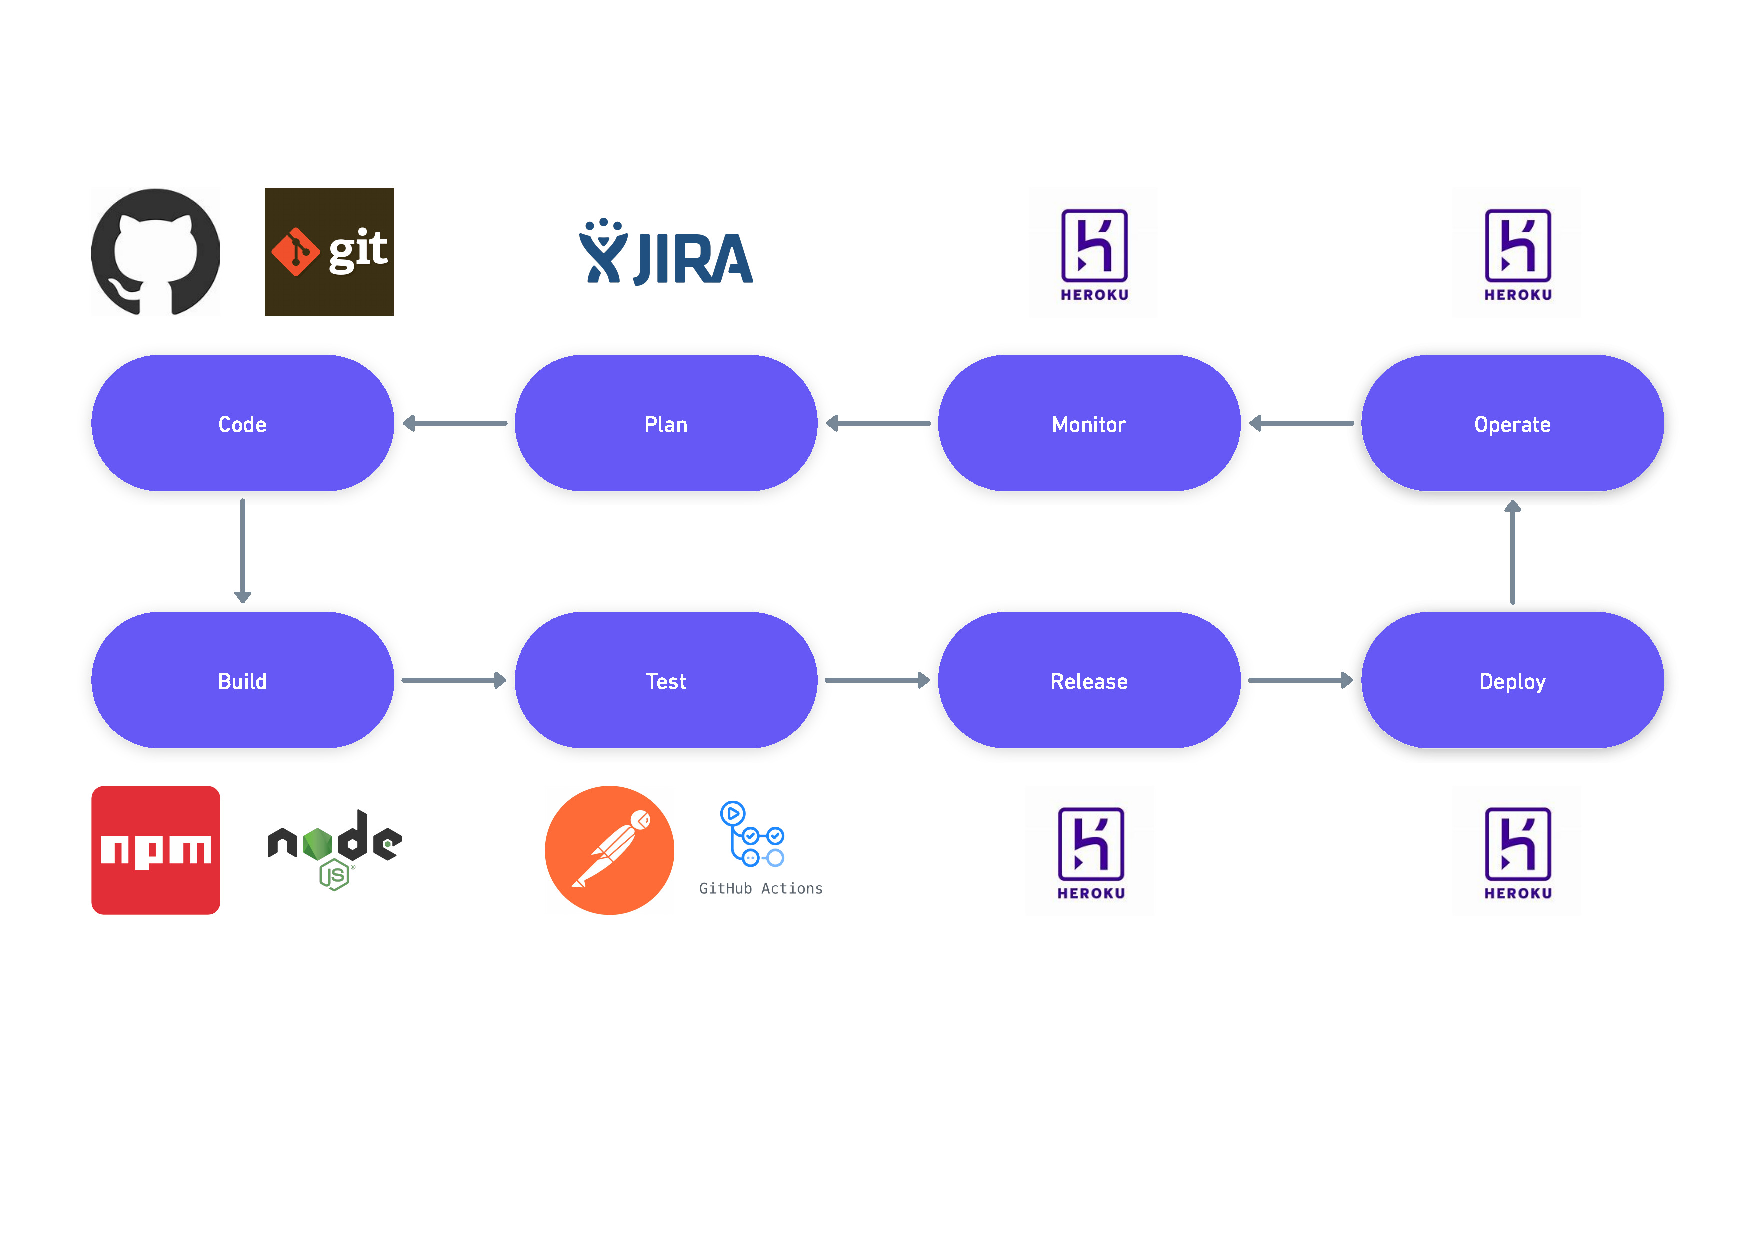
\includegraphics[width=\textwidth]{Arsitektur DevOps}
			\caption{DevOps architecture.}
			\label{fig:DevOps}
		\end{figure}
	\end{frame}

	\begin{frame}{Background}
		\begin{itemize}
			\item Pengertian
			\\DevOps merupakan metode pengembangan software dengan mengkolaborasikan \textit{software developer} dengan \textit{IT operation}.
			\item Fungsi
			\\Tujuan akhir atau \textit{goal} dari DevOps adalah untuk menciptakan lingkungan kolaborasi yang berkelanjutan untuk membawa software menjadi lebih berkualitas, lebih cepat, dan dapat diandalkan.
		\end{itemize}
	\end{frame}

	\begin{frame}{Kelebihan}
        \vspace{20pt}
		Kelebihan dari menerapkan arsitektur DevOps adalah:
		\begin{itemize}
			\item DevOps menjadi pilihan yang bagus untuk \textit{development} dan \textit{deployment} aplikasi yang cepat
			\item Merespon lebih cepat ke perubahan market untuk meningkatkan \textit{business growth} (pertumbuhan bisnis)
			\item Data dapat disentralisasikan sehingga meningkatkan konsistensi data dan mengurangi duplikasi data.
			\item DevOps meningkatkan profit bisnis dengan mengurangi waktu \textit{delivery software} dan biaya.
			\item DevOps menghilangkan proses deskriptif sehingga memberikan kejelasan mengenai \textit{development} dan \textit{delivery product}.

		\end{itemize}
	\end{frame}

	\begin{frame}{Kekurangan}
		Kekurangan dari penerapan arsitektur DevOps adalah:
		\begin{itemize}
			\item DevOps \textit{professional} atau \textit{expert} masih belum umum ditemukan.
			\item \textit{Developing} dengan DevOps mahal.
			\item Penerapan DevOps baru ke dalam industri sulit untuk dikelola dalam waktu singkat.
			\item 	Kurangnya pengetahuan mengenai DevOps dapat menyebabkan masalah pada \textit{Continuous Integration} dari \textit{project automation}.
		\end{itemize}
	\end{frame}

	\begin{frame}{Perbedaan}
		Perbedaan besar dari \textit{development} dengan DevOps dan nonDevOps yaitu:
		\begin{itemize}
			\item Kolaborasi
			\item \textit{Continuous Integration and Delivery (CI/CD)}
			\item \textit{Automation}
			\item \textit{Monitoring}
			\item \textit{Agile Development}
		\end{itemize}
	\end{frame}

	\begin{frame}{Tools}
		Tools yang digunakan:
		\begin{itemize}
			\item Git - GitHub Action
			\item Heroku
			\item Postman
		\end{itemize}
	\end{frame}

	\begin{frame}{Contoh Kasus}
		\begin{figure}[h]
			\centering
			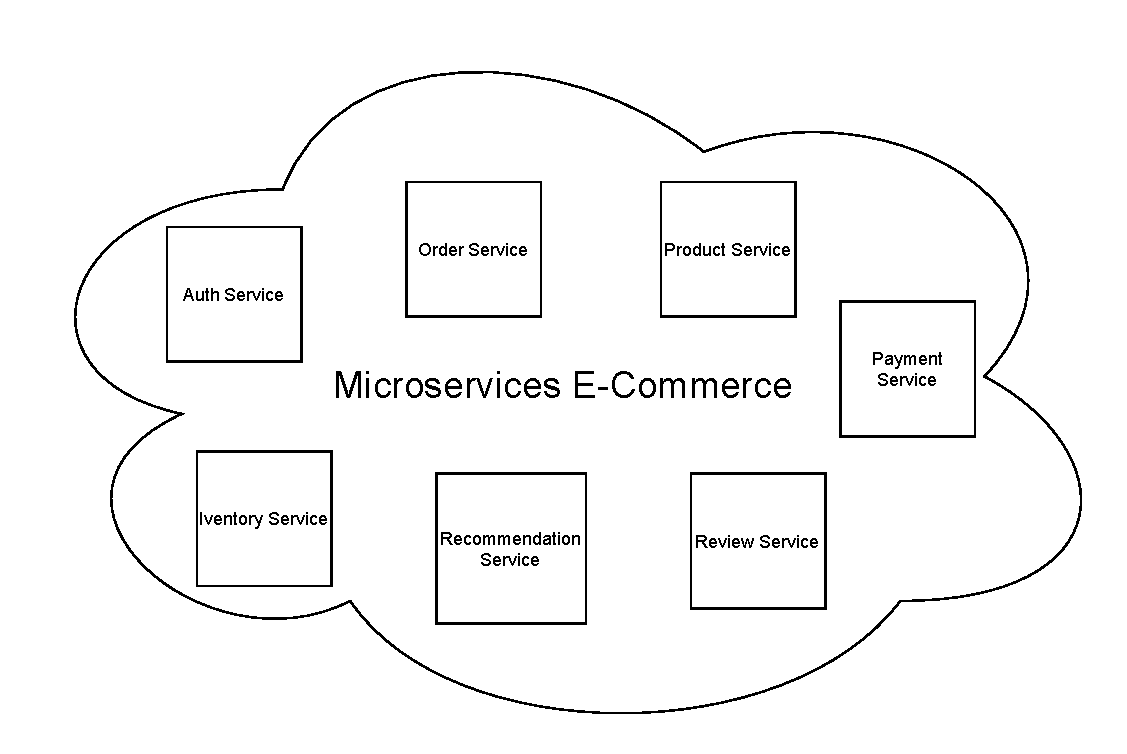
\includegraphics[width=0.6\textwidth]{Chapter-14-Studi-Kasus}
			\caption{Studi Kasus \textit{E-Commerce Microservice}.}
			\label{fig:client-server-schema}
		\end{figure}

		\end{frame}

	\begin{frame}{Links}
		Link Terkait project DevOps:
		\begin{itemize}
			\item GitHub Repository
			\\ \url{https://github.com/alfa-yohannis/software-architecture/tree/main/code/chapter14}
			\item Video Tutorial
			\\\url{https://youtu.be/My2MOkgRPwo}
		\end{itemize}
	\end{frame}

\end{document}
